\chapter{Chosen technologies}
\label{chapter:chosentechnologies}

This chapter mentions the main technologies, which I built Diplomatiq on.

\section{Spring Boot}

I like Java\footnote{https://www.java.com} because of its view of the software engineering world: its meticulous design and its the well-planned typing and interface system shows that Java is a technology which deliberately wants to be mature. Also, it is the world's most popular object-oriented programming language in 2020, according to StackOverflow~\cite{java-popularity}. Along these aspects, I was sure that I want to build Diplomatiq on a Java-based technology.

I also wanted to build Diplomatiq's back end application on a solid, production-grade solution. Although I used Spring Boot\footnote{https://spring.io} for previous hobby projects, I wanted to collect more experience with using the framework for developing an API application, for professional purposes. Spring Boot offers that it makes it easy to create stand-alone, production-grade Spring based applications that one can \textquote{just run}~\cite{spring-boot-reference-docs}.

Spring Boot offers convincing features for developers who want to build software instead of configuring and plumbing. One of Spring Boot's main characteristics is its opinionated view on starter dependencies, making initial build configuration unnecessary: one can just bootstrap a project, then start developing it without needing to select dependencies, generate code, or configure the project at all. Another important aspect is the capability creating stand-alone, self-contained Spring application with an embedded servlet container, without needing to maintain a Java application server. These two aspects, and the fact that Spring Boot is a mature, production-grade framework, convinced me easily to decide that I implement Diplomatiq's back end application with the Spring Boot framework.

\section{Angular}

I wanted to implement Diplomatiq's client application as a single-page web application, offering progressive, native-like experience to users, which is ubiquitously available with the help of only a web browser. Since the envisioned application satisfying all requirements of the Model United Nations framework would be huge in terms of code and components, a scalable, mature solution is needed, which makes use of cutting-edge web technologies, such as lazy loading application modules. Angular\footnote{https://angular.io} is a scalable, well-maintained, complete framework, and also my primary choice for larger web application projects.

I have been also developing smaller and larger Angular applications in my professional capacity for the last three years. I experienced that Angular offers a mature, complete, but customizable feature set for web applications, which aim to grow over the course of time. It also features a capable development toolset with integrations to several development environments. Since Angular is built on TypeScript\footnote{https://www.typescriptlang.org}, thus offers a competent type system, an Angular application is able to scale rapidly, while it remains maintainable.

\section{Neo4j}

Graphs are mathematically defined data structures being broadly used in several fields of computer science. Recent technologies and implementations made possible for developers to easily embed graph data models into their applications. There are numerous real-world scenarios which can be represented more efficiently as graphs (\emph{nodes} connected to each other by \emph{edges}), than with the traditional, relational approach.

Graph databases are NoSQL databases, which store data in graphs instead of the traditional, table-based approach.\footnote{The underlying data storage methods vary. There are graph databases which store graph data in relational tables, introducing another layer of abstraction between the stored physical data and the database.} In graph databases, a relationship represented as an edge in the graph is a \textquote{first-class} entity, and has the same basic storage characteristics as a node. Relationships are directly linked to entities, and therefore entities are directly linked to each other via relationships. This allows the querying of related entities to be fast, since the process does not involve lookups.

In data models where connections between data represent just as much business value as the actual data itself, it can be sensible to use graph database technologies over SQL databases. Whereas in relational databases, connections between entities rely on foreign keys and pivot tables, in graph databases they come naturally, without additional modeling needs. A (domain-specific) social network is exactly such case, where the connections value the same as data, so using a graph database was a natural decision to make.

\subsection{The property graph data model}

It is common to define graphs as a set of objects, in which some object pairs are connected to each other. In this model, an object is called \emph{vertex} or \emph{node} or \emph{point}, and a connection between two \emph{vertices} is called \emph{edge} or \emph{relation}. Connections can be detailed further by specifying their directionality, also they can be \emph{labeled} to define them even more. Similarly labeling vertices leads to the model of \emph{typed graphs}. If we assign properties to the nodes or relations, we get the model of \emph{property graphs}. Properties, as shown in \Cref{fig:property-graph}, are usually key-value pairs in the format of \lstinline{key = `value'}. Generally, keys are strings, and values represent common data types like string, integer, float, etc.

\begin{figure}[!htb]
    \centering
    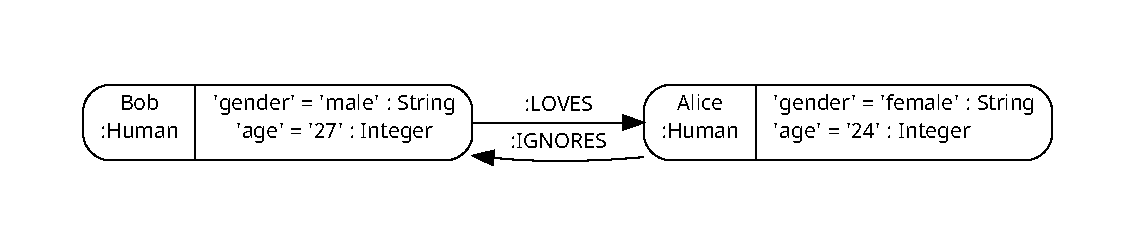
\includegraphics[width=\textwidth, trim=12mm 12mm 12mm 12mm,clip]{figures/property-graph.pdf}
    \caption{Two persons' relationship modeled with a property graph}
    \label{fig:property-graph}
\end{figure}

\subsection{The Neo4j graph database}
\label{subsection:preliminaryneo4j}

The field of graph databases has been gradually expanding in the recent years. Many vendors offer graph database solutions either based on a pure graph model or on multi-model approaches~\cite{arangodb-graph, datastax-graph, orientdb-graph}. Databases vary by query languages as well, one of the most popular being GraphQL, an open-source data and manipulation language for APIs~\cite{graphql}.

Among a handful of graph database vendors~\cite{graph-dbs}, Neo Technology's Neo4j is the most popular one~\cite{graph-dbs-raking}. It features full ACID-compliance upon a pure graph data model, contrary to other vendors' multi-model approaches. Besides Neo Technology, Neo4j is backed by the open-source community as well~\cite{neo4j-github}. There are two variants: \emph{Community Edition} and \emph{Enterprise Edition} with an extended feature set~\cite{neo4j-licensing}. Neo4j also offers a program tailored to startup companies~\cite{neo4j-startup-program}. With the help of this startup program, companies can build their applications on the Enterprise Edition of the Neo4j platform, free of charge.\footnote{Certain limitations apply: the company must have at most 50 employees and at most \$3 million annual revenue, among others~\cite{neo4j-startup-program}.}

During my Bachelor's Thesis, I had the opportunity to experience the depths of Neo4j. I refactored and extended a static code analysis software, which builds Abstract Syntax Trees, and stores them in Neo4j for running queries over the graph structure. In this project, Neo4j proved to be a stable, mature database, even usable for analysing repositories having more than 30,000 lines of code, which got mapped to an Abstract Syntax Tree with millions of nodes and even more millions of relationships. Every since then, I am confident that Diplomatiq will use Neo4j as its database platform.

\subsection{Cypher}

Cypher is a query language developed especially for graph databases by Neo Technology~\cite{neo4j-cypher}. \Cref{fig:cypher-intro} shows that the language uses a sort of ASCII-art to represent nodes and relationships: nodes are in parentheses, relationships are in brackets surrounded by relationship direction information.

\begin{figure}[!htb]
    \centering
    \lstinline{(Bob)-[:LOVES]->(Alice)}
    \caption{A basic Cypher example}
    \label{fig:cypher-intro}
\end{figure}

Cypher syntax is elegant and expressive, thus very readable. Besides using it to represent nodes and relationships, we can utilize it to access the Neo4j's indexing capabilities and stored procedures as well. Even complex pattern-matching conditions can be expressed easily and intuitively in Cypher. Although today's modern application development frameworks — adopting increasingly capable data mapping solutions — make it less and less necessary to directly interact with databases, complex queries can still involve composing database commands manually. Therefore the expressiveness and ease of use of a database query language still remains essential.

Basic querying capabilities include matching a given pattern. Patterns can include nodes, and directed relationships, and Cypher can also match by nodes' or relationships' properties. \Cref{fig:cypher-matching} shows a basic example on how to find every such relationship, in which a male human loves another female human.

\begin{figure}[!htb]
    \centering
    \lstinline|MATCH (b:Human { gender: "male" })-[:LOVES]->(a:Human { gender: "female" })|
    \caption{Basic pattern matching capabilities}
    \label{fig:cypher-matching}
\end{figure}

Inserting nodes and relationships can also be achieved in an easy and semantic way. \Cref{fig:cypher-create} shows a basic example on creating two nodes and a relationship between them.

\begin{figure}[!htb]
    \centering
    \lstinline|CREATE (b:Human { gender: "M" })-[r:LOVES]->(a:Human { gender: "F" })|
    \caption{Creating two nodes and a relationship between them}
    \label{fig:cypher-create}
\end{figure}

For avoiding inserting duplicate nodes, creation can be replaced with merging. In this case, if a node with the specified identifiers exists, it gets updated with any additional data specified by the query. Merging is similar to the create operation, as shown on \Cref{fig:cypher-merge}.

\begin{figure}[!htb]
    \centering
    \lstinline|MERGE (b:Human { gender: "M" })-[r:LOVES]->(a:Human { gender: "F" })|
    \caption{Merging to avoid creating duplicate data}
    \label{fig:cypher-merge}
\end{figure}

\section{Git and GitHub}

I have been maintaining altogether 9 projects related to Diplomatiq, all being tracked by a version control system, Git. I chose Git because of its maturity\footnote{Git has been developed since 2005~\cite{git-initial-commit}.} and popularity, and also because of the fact that this is the versioning tool that I am most experienced with. For open-source software maintenance, I chose GitHub, as it is the most popular software collaboration platform~\footnote{GitHub has over 40 million users~\cite{github-user-count}.}, and offers advanced development and project management tools, security settings, and a full-featured, integrated testing infrastructure. Also, it enables to maintain repositories under a larger unit, called organization, offering sophisticated administrative and security features. GitHub is free of charge for open-source projects~\cite{github-pricing}.

\section{Microsoft Azure}

Having relevant work experience in operating a production cloud server infrastructure, I had a concrete concept on Diplomatiq's demands on the short and on the run as well. The key aspects of choosing the platform were the following:

\begin{itemize}
\item It should provide strong cloud-based services with hybrid cloud\footnote{A hybrid cloud consists of cloud-based and on-premise infrastructure elements.} capabilities for later expansion into real-world diplomacy.\footnote{According to my knowledge, governmental and diplomatic software often require on-premise solutions.}
\item It should provide strong PaaS\footnote{Platform-as-a-Service} capabilities, and also IaaS\footnote{Infrastructure-as-a-Service} solutions.
\item It should provide options on data residency to comply with diplomatic requirements.
\item It should offer a flexible pricing model, so I can start with a smaller, cheaper infrastructure, and scale it later as Diplomatiq's production workload grows.
\item It should provide mature, integrated security solutions.
\item It should provide affordable developer support.
\end{itemize}

Considering the above, I evaluated service offerings of Microsoft Azure, Google Cloud Platform, and Amazon Web Services. Google seems to lag behind on hybrid solutions, and also seems to be the worst from the financial aspect for Diplomatiq's use cases. Even though Amazon is the oldest cloud service, it seems to lack integrated data residency solutions. Microsoft seems to offer everything Diplomatiq will need in the long run, and it proved to be the best in terms of pricing, therefore I chose Microsoft Azure as Diplomatiq's cloud server infrastructure platform.
